\documentclass[a4paper]{article}
\usepackage{amsfonts}
\usepackage{amsmath}
\usepackage{amssymb}
\usepackage{graphicx}
\usepackage{float}

\begin{document}
  
\noindent \large Auteur: Siebe Mees \\
\noindent \large Studierichting: Informatica\\
\noindent \large Oefeningenreeks 5L nr. 1.4\\

\medskip

\normalsize

$f(x)=\dfrac{x^4+3}{6x} $ op $ \left[1,2\right]$\\
  
\begin{tabular}{c|ccc}

$x$ & $1$ & & $2$ \\ \hline

$f(x)$ & $\dfrac{2}{3}$ & $+$ & $\dfrac{19}{12}$ \\

$f'(x)$ & $0$ & $+$ & $+$ \\

$f''(x)$ & $+$ & $+$ & $+$ \\ \hline

$f(x)$ & $\dfrac{2}{3}$ & $\nearrow$ & $\dfrac{19}{12}$ \\

 &  & $\smile$ &  \\

\end{tabular}\\

\begin{figure}[H]
\centering
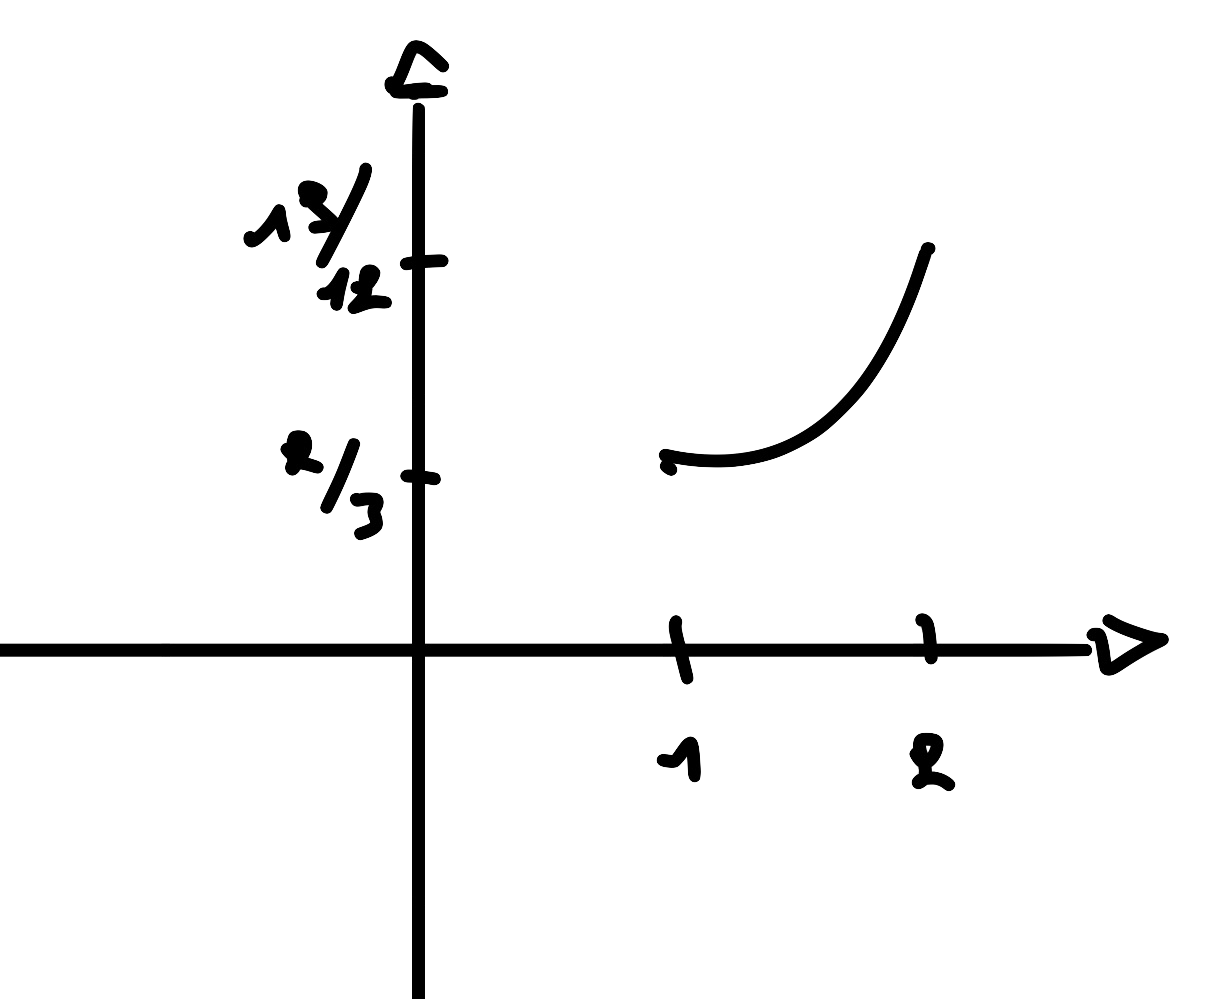
\includegraphics[width=5cm]{5L-1.4-siebe.mees.INF.png}
\end{figure}

$f'(x)=\dfrac{x^4-1}{2x^2}$\\

$S=2\pi \displaystyle\int_1^2 f(x)\sqrt{1+\left(f'(x)\right)^2} dx$\\

$=2\pi \displaystyle\int_1^2 \dfrac{x^4+3}{6x}\sqrt{1+\left(\dfrac{x^4-1}{2x^2}\right)^2} dx$\\

$=2\pi \displaystyle\int_1^2 \dfrac{x^4+3}{6x}\sqrt{1+\dfrac{(x^4-1)^2}{4x^4}} dx$\\

$=2\pi \displaystyle\int_1^2 \dfrac{x^4+3}{6x}\sqrt{\dfrac{4x^4+(x^4-1)^2}{4x^4}} dx$\\

$=2\pi \displaystyle\int_1^2 \dfrac{x^4+3}{6x}\sqrt{\dfrac{x^8+2x^4+1}{4x^4}} dx$\\

$=2\pi \displaystyle\int_1^2 \dfrac{x^4+3}{6x}\cdot\dfrac{x^4+1}{2x^2} dx$\\

$=2\pi \displaystyle\int_1^2 \dfrac{(x^4+3)(x^4+1)}{12x^3} dx$\\

$=2\pi \displaystyle\int_1^2 \dfrac{x^8+4x^4+3}{12x^3} dx$\\

$=2\pi \displaystyle\int_1^2 \left(\dfrac{x^5}{12}+\dfrac{x}{3}+\dfrac{1}{4x^3}\right) dx$\\

$=2\pi \left[\dfrac{x^6}{72}+\dfrac{x^2}{6}-\dfrac{1}{8x^2}\right]_1^2$\\

$=2\pi \left(\left(\dfrac{64}{72}+\dfrac{4}{6}-\dfrac{1}{32}\right)-\left(\dfrac{1}{72}+\dfrac{1}{6}-\dfrac{1}{8}\right)\right)$\\

$=2\pi \left(\dfrac{16}{18}+\dfrac{2}{3}-\dfrac{1}{32}-\dfrac{1}{72}-\dfrac{1}{6}+\dfrac{1}{8}\right)$\\

$=2\pi \left(\dfrac{47}{32}\right)$\\

$=\dfrac{47\pi}{16}$\\

\begin{thebibliography}{999}
%\bibitem{a} Referentie
\end{thebibliography}
\end{document} 
